\section{Agentic Variation Operators}
\label{sec:method}

\begin{figure}[t]
  \centering
    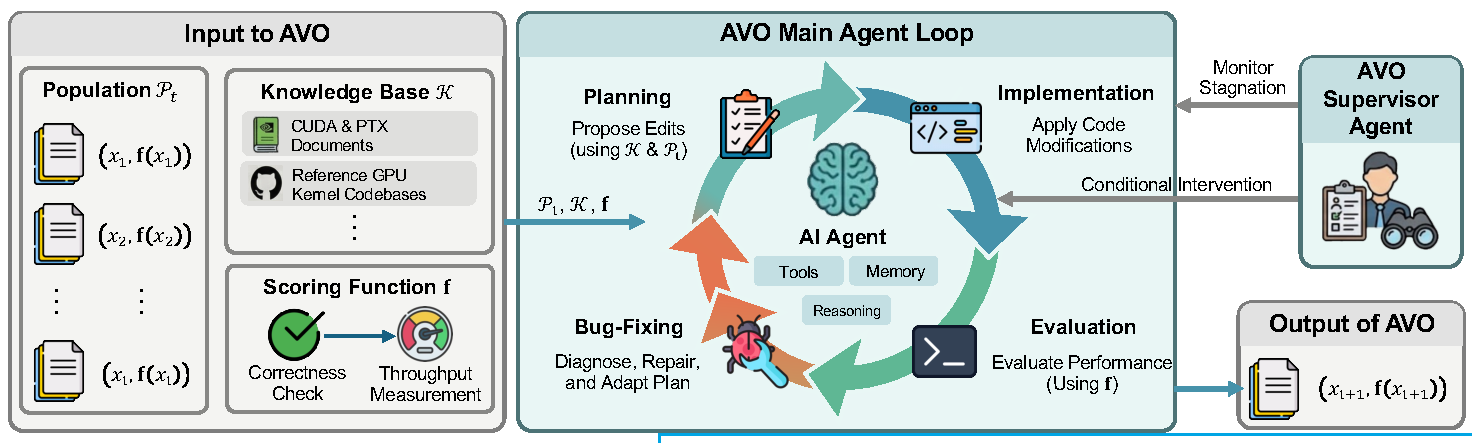
\includegraphics[width=\textwidth]{figures/overview.pdf}
  \caption{Illustration of the Agentic Variation Operator (AVO).}
  \label{fig:avo_overview}
\end{figure}

AVO consolidates the sampling, generation, and evaluation stages of evolutionary search into a single autonomous agent run, eliminating the rigid pipeline that constrains existing approaches.
Below we formalize this operator, detail what occurs within a single variation step, and describe the mechanism that enables multi-day autonomous exploration.

\subsection{Formulation}
\label{sec:method_formal}

Previous evolutionary search approaches~\citep{funsearch2024, alphaevolve2025} decompose the variation operator as:
\begin{equation}
\label{eq:evo}
\texttt{Vary}(\mathcal{P}_t) = \texttt{Generate}(\texttt{Sample}(\mathcal{P}_t)),
\end{equation}
confining the LLM to the $\texttt{Generate}$ step within a fixed pipeline.
As illustrated in Figure~\ref{fig:avo_overview}, AVO replaces this decomposition with a single autonomous agent run:
\begin{equation}
\label{eq:avo}
\texttt{Vary}(\mathcal{P}_t) = \texttt{Agent}(\mathcal{P}_t, \mathcal{K}, \mathbf{f}),
\end{equation}
where $\mathcal{P}_t = \{(x_1, \mathbf{f}(x_1)), \ldots, (x_t, \mathbf{f}(x_t))\}$ is the full lineage of solutions and their scores, $\mathcal{K}$ is a domain-specific knowledge base, and $\mathbf{f}$ is the scoring function.

In our setting, each $x_i$ is a CUDA kernel implementation (source code with inline PTX), and $\mathbf{f}$ evaluates a candidate along two dimensions: numerical correctness against a reference implementation, and throughput in TFLOPS on the target hardware. In practice, $\mathbf{f}(x_i) = (f_1(x_i), f_2(x_i), \ldots, f_n(x_i))$ is an $n$-dimensional vector and $f_j$ represents the score for test configuration $j$. 
A candidate $x_i$ that fails correctness is assigned zero score (i.e., $f_j(x_i) = 0$) regardless of throughput.
The knowledge base $\mathcal{K}$ contains CUDA programming guides, PTX ISA documentation, Blackwell architecture specifications, and existing kernel implementations including FlashAttention-4 source code.

AVO defines a family of agentic variation operators for evolutionary search. In this work, we instantiate AVO in a single-lineage autonomous run starting from a seed program $x_0$, producing a sequence of committed improvements $x_1, x_2, \ldots, x_t$. The accumulated lineage $\mathcal{P}_t$ serves as context for subsequent variation steps.

\subsection{Anatomy of a Variation Step}
\label{sec:method_step}

A single variation step in AVO, producing $x_{t+1}$ from the current lineage $\mathcal{P}_t$, is an autonomous agent loop.
The agent is a general-purpose coding agent with planning, tool use, and persistent memory (details in Section~\ref{sec:experiments}), and a single step may involve numerous internal actions.

We observe that the agent frequently examines multiple prior implementations in $\mathcal{P}_t$ within a single variation step, comparing their profiling characteristics to identify bottlenecks and opportunities, and consulting documentation in $\mathcal{K}$ to understand the relevant hardware constraints before implementing a candidate optimization.
The agent then invokes $\mathbf{f}$ to test the result.
When a candidate fails correctness checks or fails to improve on the current benchmark suite, the agent diagnoses the issue and revises its approach, repeating this edit-evaluate-diagnose cycle until it commits a satisfactory $x_{t+1}$.
This design allows the agent to adapt its optimization strategy as the search progresses: early steps may focus on structural changes informed by reference implementations in $\mathcal{K}$, while later steps can shift toward micro-architectural tuning guided by profiling feedback from $\mathbf{f}$ and patterns observed across the accumulated lineage $\mathcal{P}_t$.

In our current implementation, we persist a new committed version only when it passes correctness checks and matches or improves the benchmark score relative to the best committed version so far; unsuccessful intermediate attempts remain part of the agent’s internal search trajectory but are not added to the committed lineage.

\subsection{Continuous Evolution}
\label{sec:method_loop}

Although AVO is defined at the level of variation operators for evolutionary search, the present study evaluates a single-lineage continuous instantiation, leaving population-level branching and archive management to future extensions.
The AVO agent operates as a continuous loop that periodically produces new solutions without human intervention.
Each committed version $x_i$ is persisted as a git commit along with its score, maintaining full state continuity across the entire evolutionary process.

In long-running autonomous optimization, two failure modes can impede progress: the agent may \emph{stall} when it exhausts its current line of exploration, or it may enter \emph{unproductive cycles} of edits that repeatedly fail to improve scores.
To mitigate both, AVO incorporates a self-supervision mechanism that detects these scenarios and intervenes. Once triggered, the mechanism reviews the overall evolutionary trajectory and steers the search toward several candidate optimization directions. This conditional intervention effectively redirects exploration with fresh perspective when the current strategy has plateaued.

The 7-day run that produced our final multi-head attention kernel spanned 40 successive versions. Throughout this process, the main agent autonomously decided when to attempt new optimizations, when to revisit earlier approaches in $\mathcal{P}_t$, and when to shift strategy, while the supervisor maintained forward progress by intervening during periods of stagnation.
